In the following Experiment the effects of ego depletion on social risk with regard to con-sumer behaviour and behaviour in general will be examined. For the examination of social risk and consumer behaviour the experiment yields towards a decision between products with supposedly high versus low social risk. The second part of the questionnaire includes a scenar-io in which participants were confronted with criminal cases (judges dilemma). This test was included in order to check if ego-depletion has an effect on social-risk related decision-making in different contexts as well and not only in the context of purchase decisions, thus possibly supporting our results. Participants were provided with information of the respective perpetra-tor’s criminal record and his / her behaviour in custody. The awareness of responsibility re-garding the decision if a ‘delinquent remains in custody’ or ‘will be granted probation’ in-volves the concept of social risk.
The main components of the empirical research are divided into three subcategories. 
\begin{enumerate}[1.]
\item the depletion Task (Stroop test)
\item the self-evaluation 
\item the decision-making task (products/judges dilemma)
\end{enumerate}
Before the structure of the survey will be discussed in detail, the two parts of the question-naire have to be examined. Under the assumption that social risk is a significant factor in the decision-making process, two pre-tests of the survey were implemented. Both parts yield to the aspect of decision-making and social risk. The first and main part focuses on the decision-making process (as part of a purchase decision) under ego depletion, whereas the second part observes the decision-making process in judicial decisions under ego depletion.  

\section{Pretest}
The pre tests were designed in order to define the framework of ‘social risk’. Therefore, we conducted one survey, which yielded towards the question of social risk regarding con-sumer decisions. The other one observed the term of social risk in regard to judicial cases. Both pre tests will be more closely examined in the two following subsections.
\subsection{Consumer Choice}
The sample consisted of 34 students (21 male / 13 female) aged between 19 and 32 (m = 25,41; SD = 4,28) enrolled at the University of Hamburg. The main dependent measure for the pre test was social risk on consumer choice. Participants were presented a set of products. Each product could be distinguished by one attribute, either colour or design. Participants were randomly assigned to two groups and were shown sets of either 5 or 6 products, depend-ing on the group. Each product was presented in five different colours or designs. In the first step, participants were instructed to rank all five versions of the same product according to social risk. The following definition of social risk was given: (a) the colour or design of which they would most likely expect positive reactions of their social environment (low risk) versus (b) the product of which they would most likely expect adverse reactions of their social envi-ronment (high risk). In the second step, participants had to rank all five versions according to personal preference (in the following referred to as ‘liking scale’). The last step yielded to a consumer decision. Participants had to rank the product itself with the help of a Likert scale, with the variables being (a) social risk and (b) design as significant for a purchase decision. A sample of the questionnaire is pictured in figure 4. To emphasize the scale visually in the ques-tionnaire a grey shadowed triangle was put behind the scale.
 
\begin{figure}[h!]
\center
	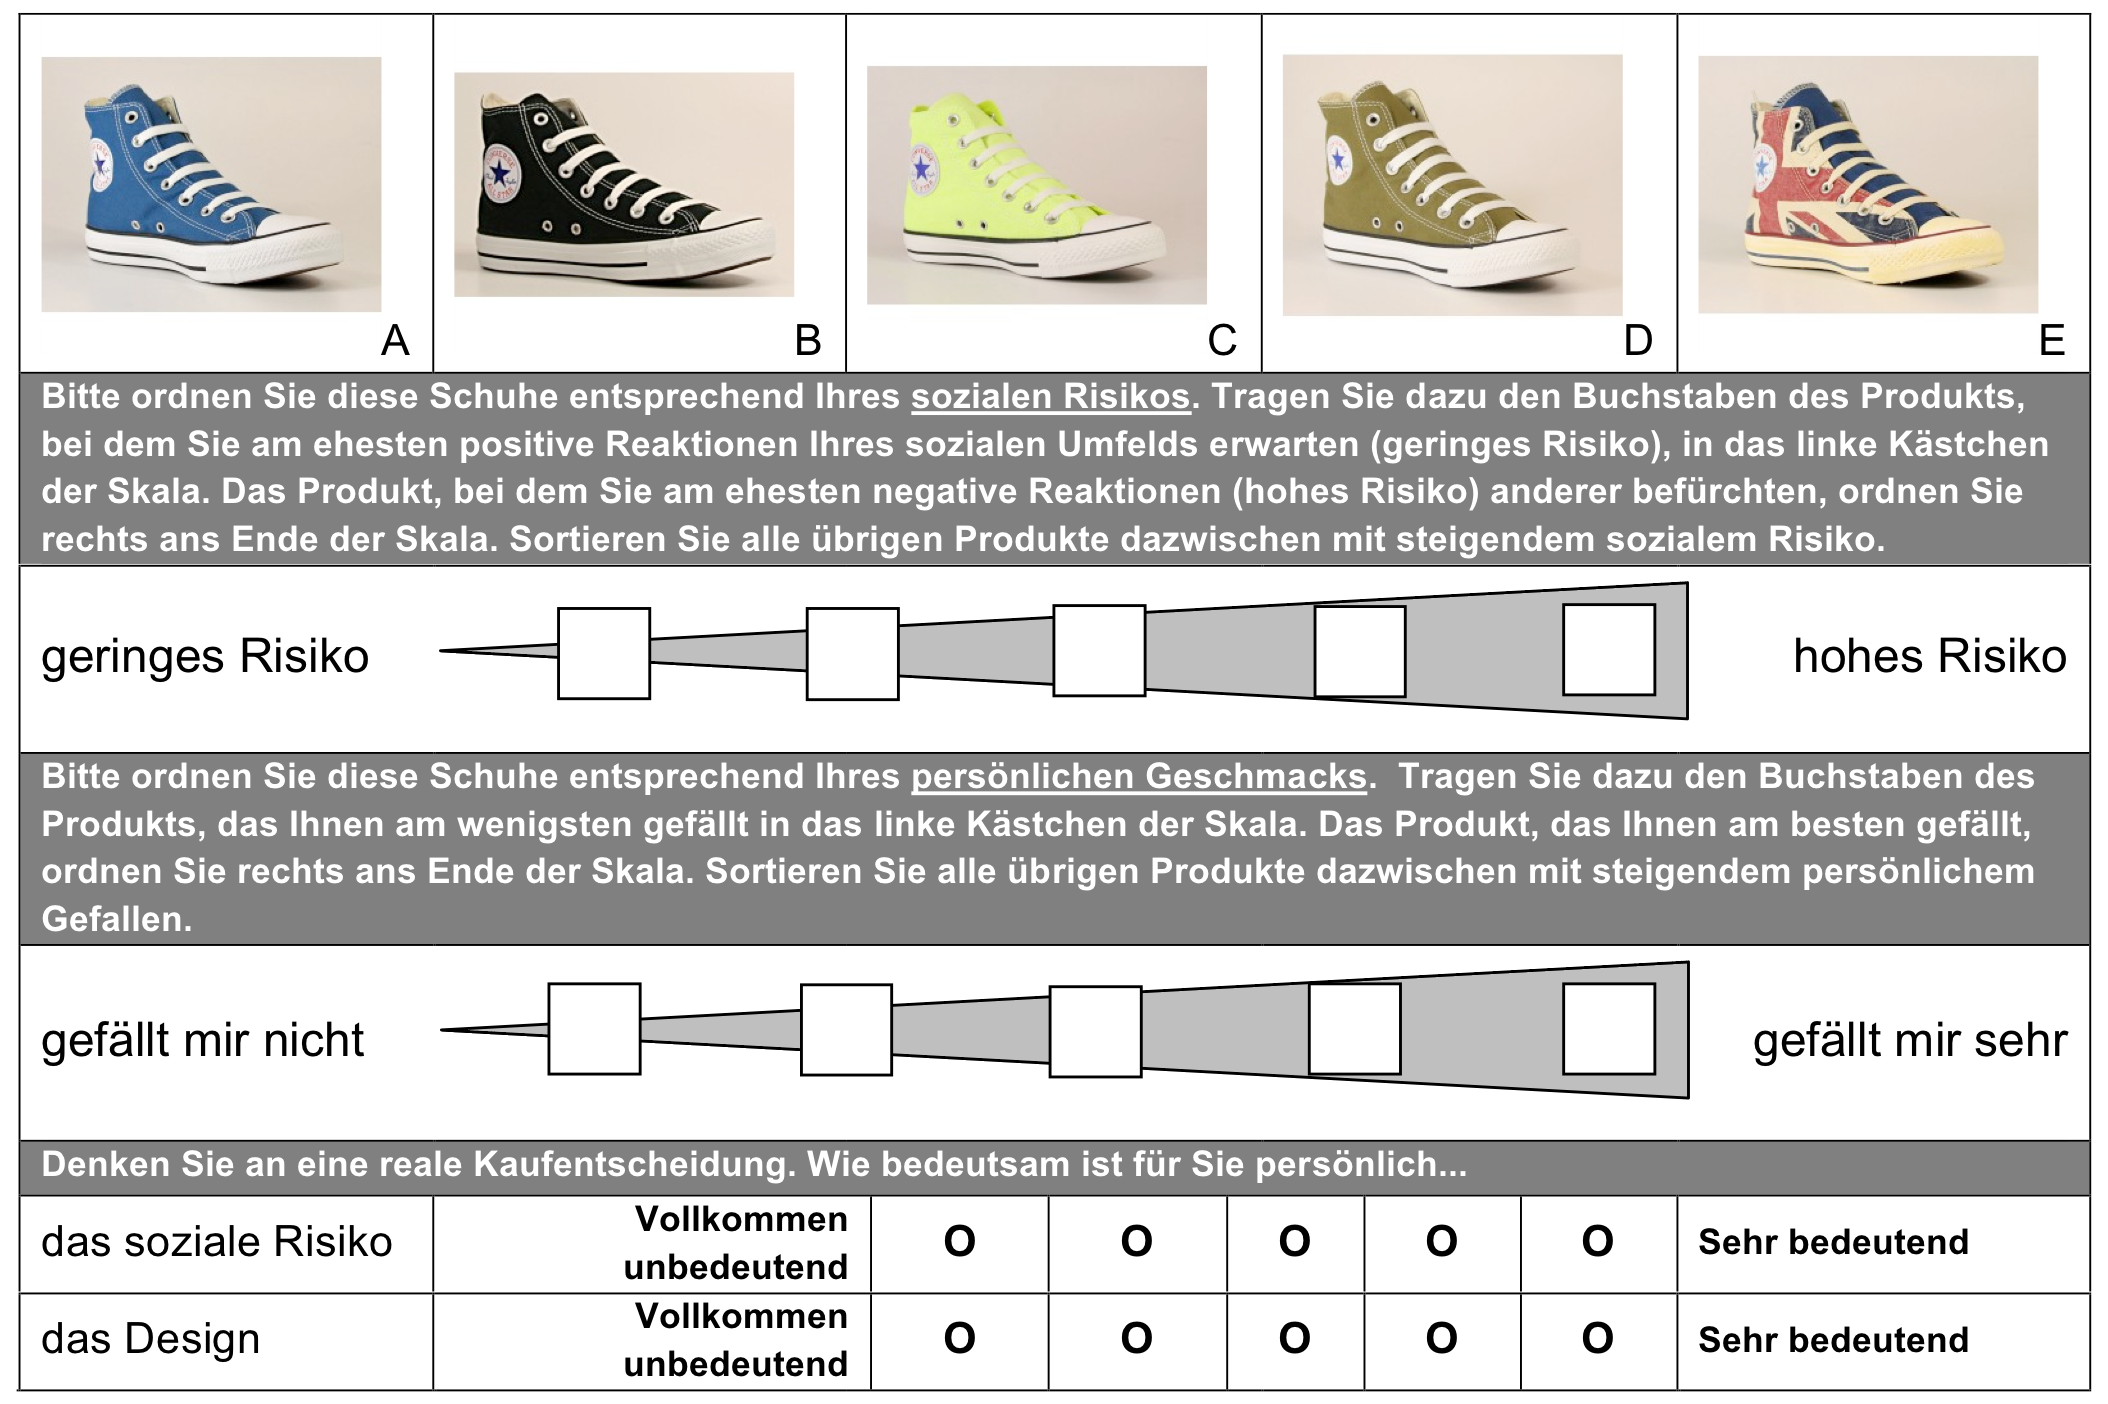
\includegraphics[width=0.9\textwidth]{images/sample.png}
  \caption{Figure 4 sample of the pre test (own design)} \label{fig:sample}
\end{figure}
Products were chosen to be part of the final questionnaire based on the premise that they pro-vided an approximately equivalent liking and a preferably diverse social risk. Four of the elev-en products complied with our expectations (shoes, sofa, wine, MP3 player and car).  
Figure 5 displays the five alternatives regarding the product ‘shoes’. The variation ‘black’ with a strong ‘low-risk’ rating and the variation ‘yellow’ with a weak ‘social-risk’ rating would in-dicate the maximum of difference between the variable ‘social-risk’. The ‘liking’ rate of these two product variations, however, show also the highest deviation. Therefore, we decided to select the product ‘shoe’ with the attribute ‘blue’ (SR = 2.06; liking = 3.50) as the low social risk, and the ‘union jack’ (SR =  4.12; liking = 2.87) as the high social risk alternative. In addi-tion the product choices regarding the variable ‘liking’ corresponded more strongly with each other. 

\begin{figure}[h!]
\center
	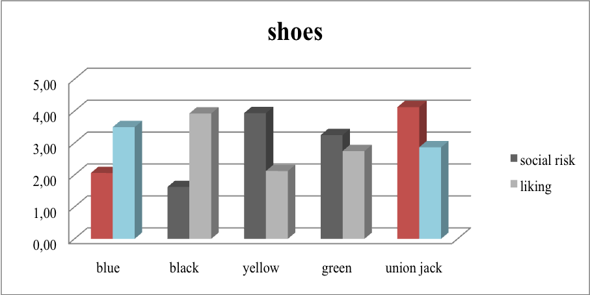
\includegraphics[width=0.9\textwidth]{images/shoespretest.png}
  \caption{Figure 5 results of pre test (shoes)} \label{fig:shoespretest}
\end{figure}